\documentclass{article}

\usepackage{graphicx}
\usepackage{tikz}
\usepackage{tikzsymbols}
\usetikzlibrary{calc,patterns,shapes.geometric}
\pagestyle{empty}
\usepackage[margin=0pt]{geometry}
\geometry{papersize={14in,12in}}

\def\centerarc[#1](#2)(#3:#4:#5){\draw[#1] ($(#2)+({#5*cos(#3)},{#5*sin(#3)})$) arc (#3:#4:#5);}

\begin{document}
	\begin{figure}
		\centering
		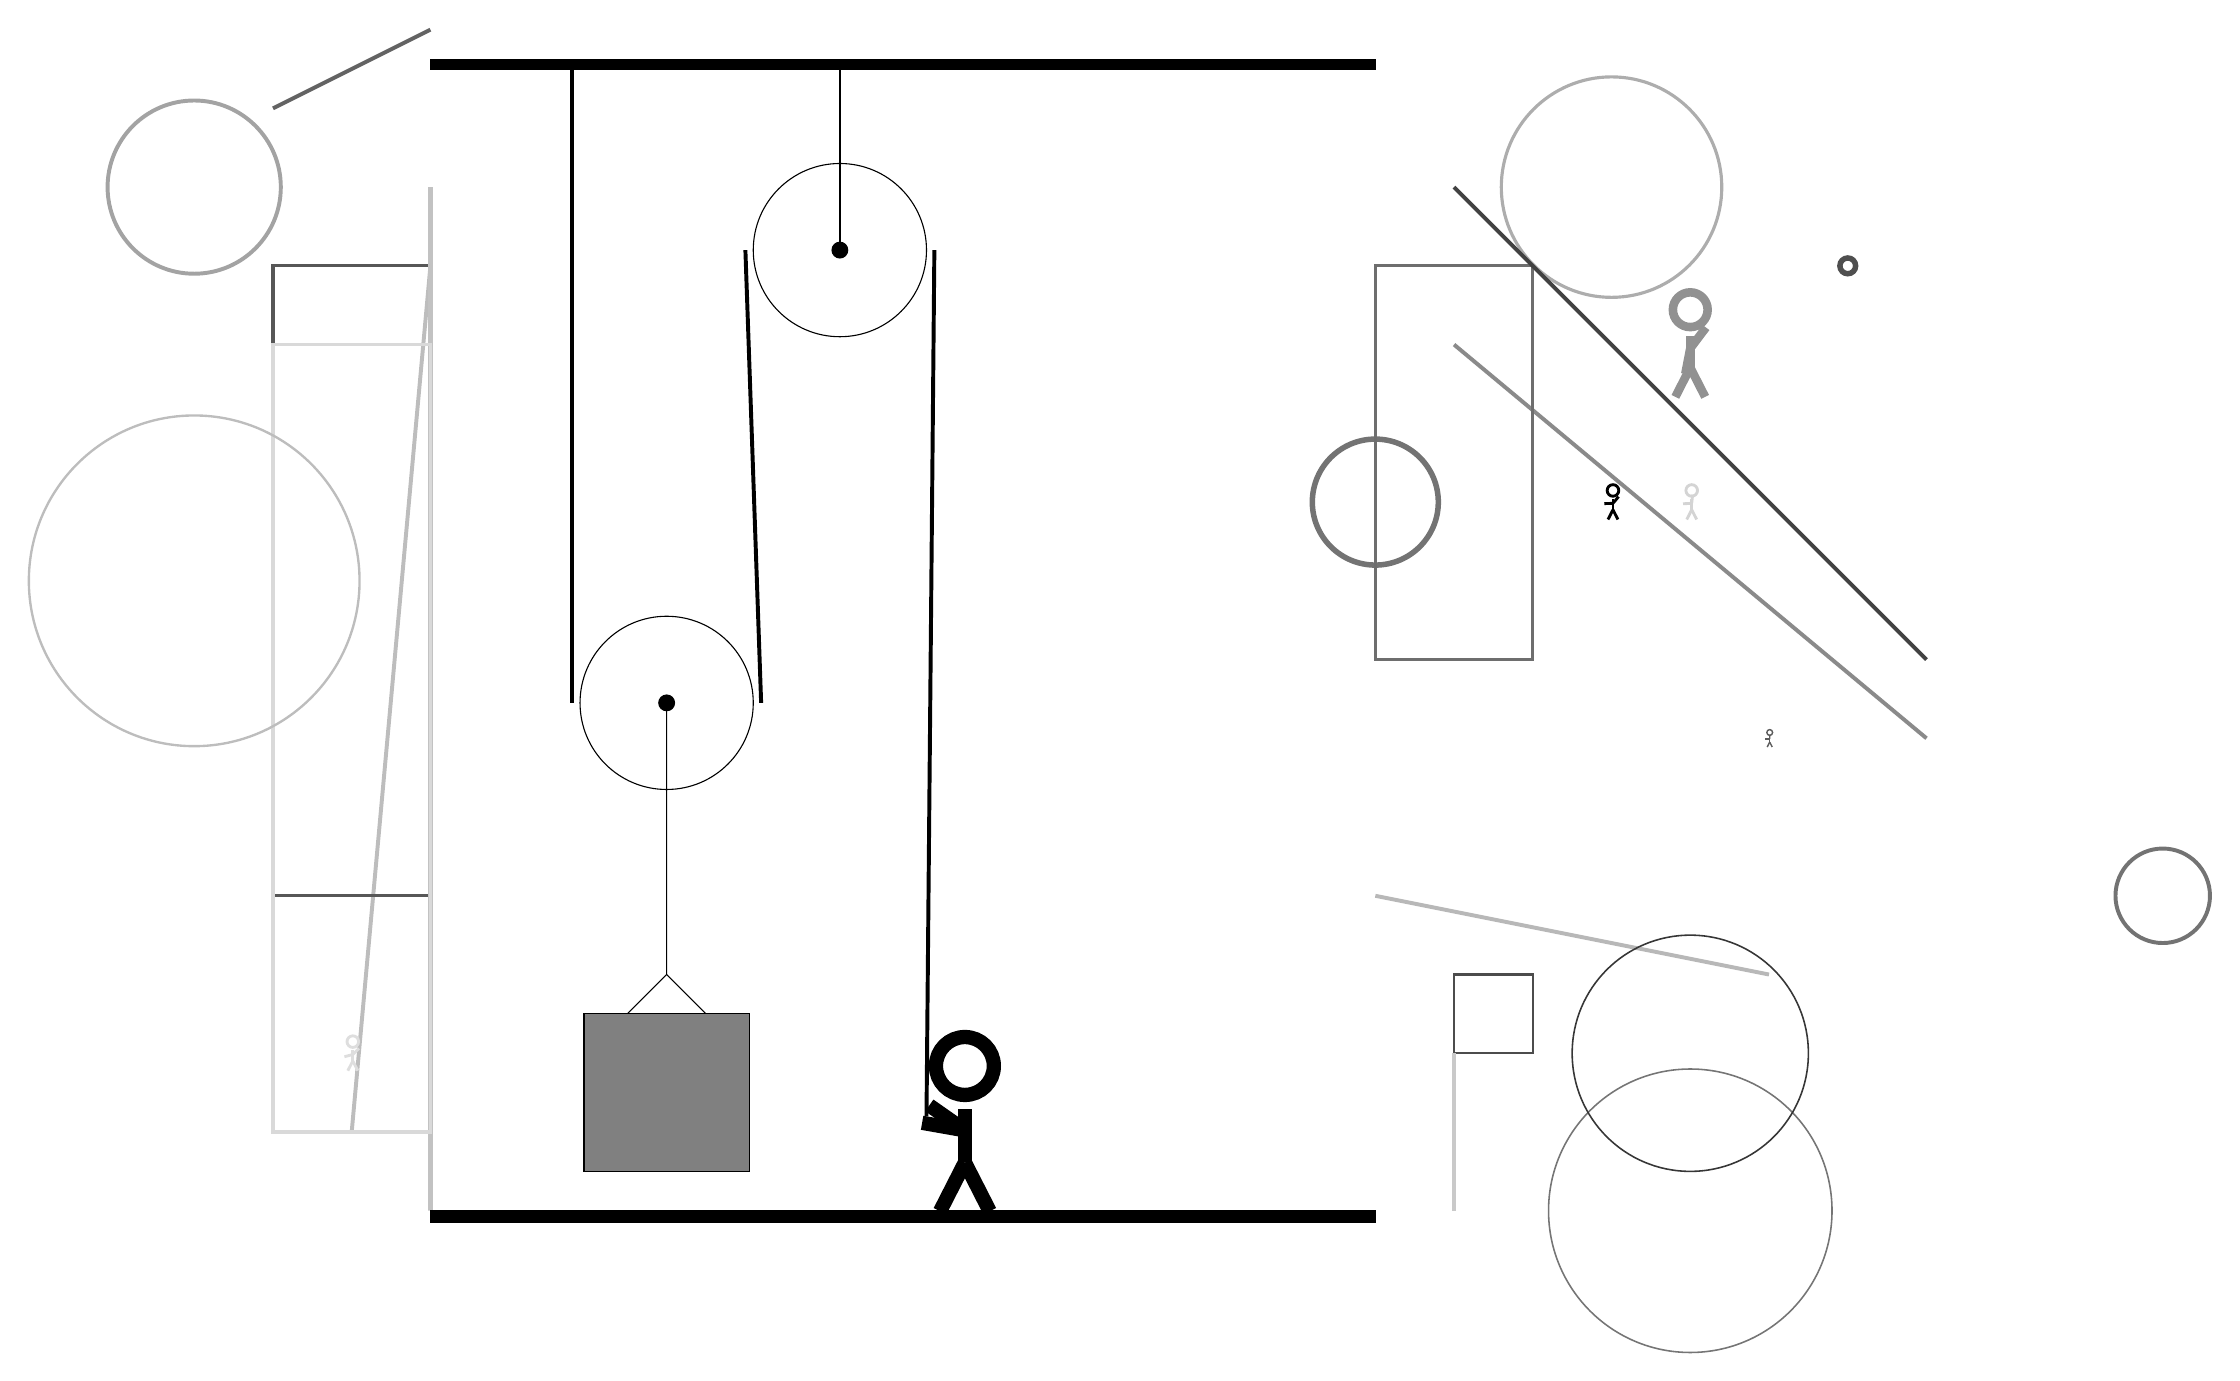
\begin{tikzpicture}
			%%%%% START %%%%%
			
			\draw[fill=black] (-2, 11.5) rectangle (10, 11.625);
			
			\draw (3.2, 9.2) circle (1.1);
			\draw[fill=black] (3.2, 9.2) circle (0.1);
			\draw[thick] (3.2, 9.2) -- (3.2, 11.5);
			
			\draw[line width=0.5mm, color=black!26](-2, 9) -- (-3, -2);
			
			\draw [line width=0.7mm, color=black!55](10, 6) circle (0.8);
			\draw[line width=0.5mm, color=black!46](11, 8) -- (17, 3);
			\node[line width=0.6mm, color=black!100] at (13, 6) {\Strichmaxerl[2][2][50]};
			\draw[line width=0.3mm, color=black!70] (12, -1) rectangle (11, 0);
			\node[line width=0.4mm, color=black!43] at (14, 8) {\Strichmaxerl[6][79][53]};
			\draw[line width=0.4mm, color=black!66] (-2, 1) rectangle (-4, 9);
			\draw [line width=0.5mm, color=black!36](-5, 10) circle (1.1);
			\draw [line width=0.4mm, color=black!32](13, 10) circle (1.4);
			\draw[line width=0.6mm, color=black!24] (-2, 10) rectangle (-2, -3);
			\draw[line width=0.5mm, color=black!61](-4, 11) -- (-2, 12);
			\draw [line width=0.5mm, color=black!55](20, 1) circle (0.6);
			\draw[line width=0.3mm, color=black!82] (-4, 1) rectangle (-4, 8);
			\draw[line width=0.4mm, color=black!15] (-2, 8) rectangle (-4, -2);
			\draw [line width=0.7mm, color=black!26](13, -1) circle (0.0);
			\draw [line width=0.2mm, color=black!54](14, -3) circle (1.8);
			
			\node[line width=0.6mm, color=black!17] at (14, 6) {\Strichmaxerl[2][3][84]};
			\draw [line width=0.3mm, color=black!26](-5, 5) circle (2.1);
			\draw[line width=0.4mm, color=black!57] (10, 9) rectangle (12, 4);
			\node[line width=0.4mm, color=black!13] at (-3, -1) {\Strichmaxerl[2][15][45]};
			\draw [line width=0.7mm, color=black!69](16, 9) circle (0.1);
			
			\draw[line width=0.5mm, color=black!21](11, -3) -- (11, -1);
			
			\draw[line width=0.5mm, color=black!28](15, 0) -- (10, 1);
			\draw [line width=0.2mm, color=black!79](14, -1) circle (1.5);
			\node[line width=0.3mm, color=black!64] at (15, 3) {\Strichmaxerl[1][0][89]};
			\draw[line width=0.5mm, color=black!74](11, 10) -- (17, 4);
			
			
			\draw (1, 3.45) circle (1.1);
			\draw[fill=black] (1, 3.45) circle (0.1);
			
			\draw (1, 3.45) -- (1, 0.0) -- (0.5, -0.5);
			\draw (1, 0.0) -- (1.5, -0.5);
			\draw[fill=black!50] (-0.05, -0.5) rectangle (2.05, -2.5);
			
			\draw[line width=0.5mm] (-0.2, 11.5) -- (-0.2, 3.45);
			\centerarc[line width=0.5mm](1, 3.45)(180:360:1.2000000000000002);
			\draw[line width=0.5mm](2.2, 3.45) -- (2.0, 9.2);
			\centerarc[line width=0.5mm](3.2, 9.2)(0:180:1.2000000000000002);
			\draw[line width=0.5mm](4.4, 9.2) -- (4.3, -1.8);
			
			\node at (4.7, -1.9) {\Strichmaxerl[10][-35][170]};
			
			\draw[fill=black] (-2, -3) rectangle (10, -3.15);
			
			%%%%% END %%%%%
		\end{tikzpicture}
	\end{figure}	
\end{document}